\documentclass[Japanese]{dicomopapers}
%\documentclass[Japanese,noauthor]{dicomopapers}

\usepackage[dvipdfmx]{graphicx}
\usepackage{latexsym}

\def\Underline{\setbox0\hbox\bgroup\let\\\endUnderline}
\def\endUnderline{\vphantom{y}\egroup\smash{\underline{\box0}}\\}
\def\|{\verb|}

\def\newblock{\hskip .11em plus .33em minus .07em}

\begin{document}

% 和文表題
\title{圧力センサ搭載ヘルメットを用いた\\個人識別手法の提案}
% 英文表題
%\etitle{DICOMO2019 Paper Format (optional)}

% 所属ラベルの定義
\affiliate{RU}{立命館大学 情報理工学部}
\affiliate{JST}{JSTさきがけ}

\author{藤井 敦寛}{ATSUHIRO FUJII}{RU}
\author{村尾 和哉}{KAZUYA MURAO}{RU, JST}

\begin{abstract}
近年,四輪車において広く普及しているスマートキーシステムが,徐々に二輪車でも採用されつつある.しかしこのシステムは電子キーを所持しておく必要があり,鍵の紛失の恐れ,更には鍵の盗難による車両盗難のリスクがある.そこでヘルメットを鍵の代用とすることが可能であれば,二輪車のヘルメットロックに装備しておくことで,所有者は身体一つで乗車が可能となり,先述のリスクも回避できると考えた.\par
本研究ではその前段階として,圧力センサを搭載したヘルメットを装着することで個人識別する手法を提案する.識別の要素には,特徴があり複製が難しく,さらに視界を遮ることなく取得できるものとして頭部形状を選択した.頭部状態の測定にヘルメットを用いている先行研究は筆者らの知る限りは存在せず,頭部装着型デバイスとしても新規性がある.この手法では,ヘルメットに搭載した32個の圧力センサから得られたセンサ値をベクトルとして扱い,事前に登録フェーズで蓄積しておいた所有者のセンサデータ群とのマハラノビス距離を計算し,閾値を用いて識別を行う.\par
本手法で用いるデバイス,およびソフトウェアを設計,実装し評価実験を行った.プロトタイプデバイスは市販のフルフェイスヘルメットをセンサを取り付け加工し,マイコンに配線することで設計した.また,解析用のソフトウェアはPythonのscikit-learnを使用し,マハラノビス距離を計算,閾値を移動しながら評価指標であるFAR,FRR,EERを求めるよう設計した.実装後,評価実験用に被験者9人に20回ずつヘルメットを装着し,2秒間のセンサ値を収集した.このデータセットからマハラノビス距離を用いて識別を行い,被験者ごとに結果を計算した.さらに被験者全員の結果の平均値を求め,全体での結果としてEERが約7.8\%という数値が得られた.
\end{abstract}

% 表題などの出力
\maketitle

% 本文はここから始まる
\section{はじめに}
近年販売されている四輪車の多くはスマートキーシステムを導入している.スマートキーシステムは電子キーをポケットなどに入れて接近すると,それを感知しドアの施錠,解錠やエンジンの始動をボタン一つで操作できるようにする機能である.このシステムは二輪車においても導入されつつある.二輪車におけるスマートキーシステムも同様に,電子キーを所持しておくことで,キーシリンダーにキーを挿し込む手間なくラゲッジスペース(メットイン)の解錠やエンジンの始動が可能になるという機能である.しかしながら,このシステムはキーを所持しておかなければならず,鍵の紛失の恐れ,更には鍵の盗難による車両盗難のリスクがある.\par
本研究では,圧力センサを搭載したヘルメットを装着することで,頭部形状に基づき個人識別をする手法を提案する.二輪車での走行で必要であるヘルメットを用いた本人認証が実現できれば,既存のキーの問題点を解決できると考えた.予め車両とリンクしてあるヘルメットをキーの代わりとして,二輪車のヘルメットロックに装備しておく.すると,利用者は身体一つで乗車できるため,鍵の紛失のリスクを減少させることができる.そして,利用者はヘルメットを被ることで認証を行う.車両の持ち主がヘルメットを被った場合はエンジンの始動を可能にする.その一方で,車両の持ち主以外がヘルメットを被った場合はエンジンの始動ができないような機能を実現することで,車両盗難のリスクを減少させることができる.また,認証の要素には各個人ごとに特徴があり,かつ複製が難しい部位を用いる必要がある.本研究で用いる頭部形状は人により異なり特徴が存在する上,身体部位としても大きい部位であるため,複製するには大掛かりな器具が必要となることが想定される.以上の理由から,認証要素に有効だとして選択した.\par
以降,2章では関連研究を紹介する.3章では提案手法について述べ,4章では提案手法の精度を評価し,最後に5章で本研究をまとめる.

\section{関連研究}
\subsection{個人識別の手法}
個人識別には様々な手法が存在し,現在も改良が続いている手法も少なくない.\par
当麻らはステレオカメラを用いた顔認証システムを提案している\cite{face}.既存の顔認証システムではカメラに意識して顔を向ける必要があった.その問題を解決するため,少数の正面を向いていない顔画像から正面顔画像を作成し,個人認証を行う手法を提案した.このシステムでは,1台のステレオカメラを用いてステレオマッチング処理を行い顔の3次元形状を再構成し,それらを回転させることで正面顔の3次元モデルを生成する.そしてこれを2次元画像に戻すことで正面顔画像を作成する.復元された正面顔画像とデータベースにある画像とを比較するという流れで個人認証を行っている.顔認証を行うには,ヘルメットを装着する前である必要がある.少数のカメラであれば,車両に取り付けることでシステムを実装することが可能だ.佐藤らは掌紋認証を装備したインテリジェントドアノブシステムの開発を提案している\cite{door}.認証に特別な動作を必要とする煩わしさを解決するため,ドアノブにカメラを装着し掌紋の画像を取得する.このシステムの場合,二輪車のハンドル部分にカメラを搭載することで実装が可能だろう.しかしながら,二輪車では悪天候や夜間における使用,耐久性も考慮しなければならない.したがって,カメラを車両に取り付ける必要のある手法は向かないだろう.\par
成ケ澤らは加速度センサとジャイロセンサを併用したスマホ回しによる認証手法を提案している\cite{acceleration}.この手法では,スマートフォン内臓の加速度センサとジャイロセンサを用い,ユーザがスマートフォンを手のひらの上でY軸を中心に回転させる動作を行うことで,その加速度と角速度の特徴量から認証する.手を動かすのみで認証動作を行うことができるため狭い空間でも認証を行える.ヘルメットに加速度センサとジャイロセンサを搭載することで,ヘルメットを被るまでの動作の加速度と角速度の特徴量から同様の手法が実装できる可能性がある.しかしながら,急いでいて動作が速くなったり,雨でヘルメットの内装が濡れないよう気をつけながら被る場合など,特徴量が変化してしまう状況が考えられる.屋外環境の変化を考慮すると,ヘルメットを静止させたまま識別が可能な手法が有効だろう.\par
白川らは虹彩と目の周辺画像を統合して認証する手法を提案している\cite{iris_eye}.虹彩認証は高画質の画像を必要とし,至近距離で認証を行う必要があり,被認証者に負担を与えてしまう.そこで目頭や目尻,まぶたの形などに個人差が存在することに注目し,目の周辺の分割画像を利用して目の周辺認証を行い,虹彩と統合する認証を提案した.しかし,虹彩や目の周辺の分割画像を取得するには目の前にカメラを設置する必要がある.そのためヘルメットに取り付けると,視界を遮る恐れがあり危険だ.一方で,頭部形状は視界を遮ることなく取得できる.岸里らは口唇領域の動きの画像認識を用いたスマートデバイス向けパターンロックシステムを提案している\cite{mouth_pattern}.スマートフォンやタブレット端末のパターンロック認証は,肩越しに画面を覗き見るショルダーハックや,画面に残った脂の跡を読み取ることによって,認証キーを盗まれてしまうリスクを持つ.そこで手の指の代わりに,端末のカメラで口唇領域の動きを認識し,画面に触れることなく認証を行うシステムを提案した.視線や瞬きは拘束せずに頭部を動かさない状態で,自由度の高い可動部位は口唇のみであることを応用し,画面に触れることなく,手の指を用いる場合と近い感覚で認証処理を実現している.口唇領域の画像であれば視界を遮らずに撮影できるが,ヘルメットの口元の空間は限られるため,1個のカメラで口唇領域の動きを判別するのは難しいだろう.しかし,カメラ数を増加させるとヘルメットの重量増加に繋がる恐れがある.また,パターン入力を行う煩わしさも発生する.越前らは写真からの指紋復元の脅威とその対策技術を提案している\cite{finger_print}.指紋認証には複製の恐れがあり,少ない写真でも簡易に複製が可能である.そのため,(1)指に着用することで撮影された指紋画像と登録指紋との照合ができない(2)一方で,指に着用しても接触式の指紋センサを経由すれば登録指紋との照合は可能という2つの要件を満たす手段を検討し,指へジャミングパターンを装着する手法を提案した.しかしこの対策技術では,常にジャミングパターンを指に装着しておく必要があり現実的ではない.そのため,依然として指紋の複製のリスクが残っていると言える.一方で頭部形状の複製は,立体形状を正確に把握する必要があり,多量の写真を要するため複製は困難となる.

\subsection{頭部装着型デバイス}
田中らはメガネ型デバイスを用いた経皮水分蒸散量の常時測定システムを提案している\cite{glasses}.皮膚状態の診断には経皮水分蒸散量などの定量的な指標が用いられるが,測定には高価な機器が必要で,また定常的な測定はできない.そこで,定常的に測定を行い皮膚の健康維持を支援するため,メガネ型デバイスに2つの温度・湿度センサを装着し,皮膚状態の評価指標である経皮水分蒸散量の常時測定を行うシステムを提案した.石井らは人間の対面コミュニケーション能力を拡張するマスク型デバイス「HappyMouth」を提案している\cite{happymouth}.このシステムでは,マスクに小型ディスプレイが内蔵されており,口元での映像提示を行うことができる.映像提示の機能として,ユーザが自分の好みの口を選択して表示する機能,ユーザの発話をテキスト化して字幕表示する機能,ユーザの発したキーワードをインターネットで画像検索した結果を表示する機能がある.新島らは左右の側頭筋の筋活動を測定することができる,導電性高分子の布電極を用いた帽子型筋電センサhitoeCapを提案している\cite{cap_sensor}.食事や睡眠や運動などの日々の生活の様々な場面で活動する,咀嚼筋の一つである側頭筋の筋電データを測定すれば,ユーザのライフログとして活用できると考えられる.これらの研究はいずれも頭部に装着するデバイスであり,様々なデバイスが提案されている.しかしながら,頭部装着型デバイスとしてヘルメットを用いた例は,筆者の知る限りは存在しない.

\subsection{頭部状態の認識}
近年注目されているヒアラブルデバイスにおいて求められる機能の一つとして,手や視界を占有することのないデバイス操作機能が挙げられる.既存の製品や既存研究では認識精度や認識できるジェスチャの種類,頑健性などの点で課題が残る.これらの課題の解決のために雨坂らは首,顎,顔の状態 (頭部状態) に伴って外耳道が変形することに着目し,外耳道インパルス応答を測定することで頭部状態を認識する手法を提案した\cite{ear}.山下らは口周辺の形状変化による状況認識手法を提案している\cite{mouth}.状況の変化に関して口周辺の動作に着目すると,感情や咀嚼といった様々な情報が含まれており,これらを認識することで感情の記録や,咀嚼カウントによる肥満防止など,新たなコンテキストアウェアサービスが提供できる.そこで日常生活での利用を想定し,安価な付け髭型デバイスを用いた,口周辺の形状変化によるコンテキスト認識手法を提案した.これらの研究は表情や動作など,動的な情報を取得するものであり,本研究では静的な頭部形状そのものの特徴を取得するという点で異なる.

\section{提案手法}
本章では提案手法の詳細を述べる.本研究はヘルメットをキーの代わりとして用いるために,圧力センサを搭載したヘルメットを装着し,装着者の頭部形状を取得することで個人識別を行う手法を提案する.本手法では個人識別を行うために,着座状態でヘルメットを装着している環境を想定している.今回は研究段階として,データは全て収集後のものを用いている.

\subsection{システム構成}
システム構成を図\ref{system}に示す.学習データ群および新たにプロトタイプデバイスから得られるデータは,32個のセンサ値であり32次元のベクトルとして扱う.\par

\begin{figure}[!t]
  \begin{center}
    \includegraphics[width=1\linewidth]{figure/system.eps}
  \end{center}
  \caption{システム構成}
  \label{system}
\end{figure}

提案するシステムではあらかじめ学習フェーズとして,所有者の頭部データを複数採取しておく.このデータ群に対し,プロトタイプデバイスから得られたベクトルからのマハラノビス距離を計算する.マハラノビス距離とは統計学で用いられる一種の距離である.これは多次元のデータに対しても使用できる.ここで仮に,データがn次元の連続ベクトルであるとして,得られた多変数ベクトルのデータ列を
\[
  x^m = x_1, x_2, \ldots, x_m
\]
として,i番目のデータは
\[
  x_i = \left(
        \begin{array}{c}
            x_{i,1} \\
            x_{i,2} \\
            \vdots \\
            x_{i,n}
        \end{array}
    \right)
\]
と表すとき,その平均値ベクトル$\mu$と分散共分散行列$\Sigma$は以下のように求められる.
\begin{eqnarray*}
  \mu &=& \frac{1}{m}\sum_{i=1}^{m}x_i \\
  \Sigma &=& \frac{1}{m}\sum_{i=1}^{m}(x_i-\mu)(x_i-\mu)^T
\end{eqnarray*}
ここで閾値を$\theta$と置き,未知のユーザの入力データ$x$に対して,
\[
  \theta < \sqrt{(x_i-\mu)^{T}\Sigma^{-1}(x_i-\mu)}
\]
を満たすとき入力データ$x$は異常値,すなわち他人の頭部データだとして拒否する.その一方で入力データ$x$に対して,
\[
  \theta \geq \sqrt{(x_i-\mu)^{T}\Sigma^{-1}(x_i-\mu)}
\]
を満たした場合,入力データ$x$は正常値であり,本人の頭部データだとして認証する.

\subsection{実装}
\subsubsection{ハードウェア}
提案手法に用いる,圧力センサを搭載したヘルメットを実装した.このプロトタイプデバイスの全体図を図\ref{met_over}に,デバイス構成を図\ref{device}に示す.センサ値を正しく取得するには,センサとヘルメット装着者の頭部が密着している必要がある.そのため,フルフェイス型のB\&B社製BB100フルフェイスヘルメットを用いた.次にプロトタイプデバイスの内部を図\ref{met_in}に示す.今回用いたヘルメットはフリーサイズであり,また内装の脱着が困難であったため,頭頂部の内装を取り外して,新たに厚みのあるウレタンスポンジを取り付けた.ここで,図\ref{sensor}のようにウレタンスポンジの中央部に切り込みを入れ,インターリンク エレクトロニクス社製のFSR402,FSR402 ShortTailを挿し込むことで圧力センサを実装した.この圧力センサは頭頂部に4個,頭頂部周囲に16個,後頭部に6個,左右チークパッド部に6個の合計32個を搭載してあり,ヘルメット外部に取り付けた10KΩの抵抗を配線してあるプリント基板を経由して,Arduino MEGA2560 R3のアナログ入力ポートに接続した.センサ1つあたりの回路図を図\ref{circuit}に示す.この回路を,図\ref{print}に示したプリント基板で並列に接続した.

\begin{figure}[!t]
  \begin{center}
    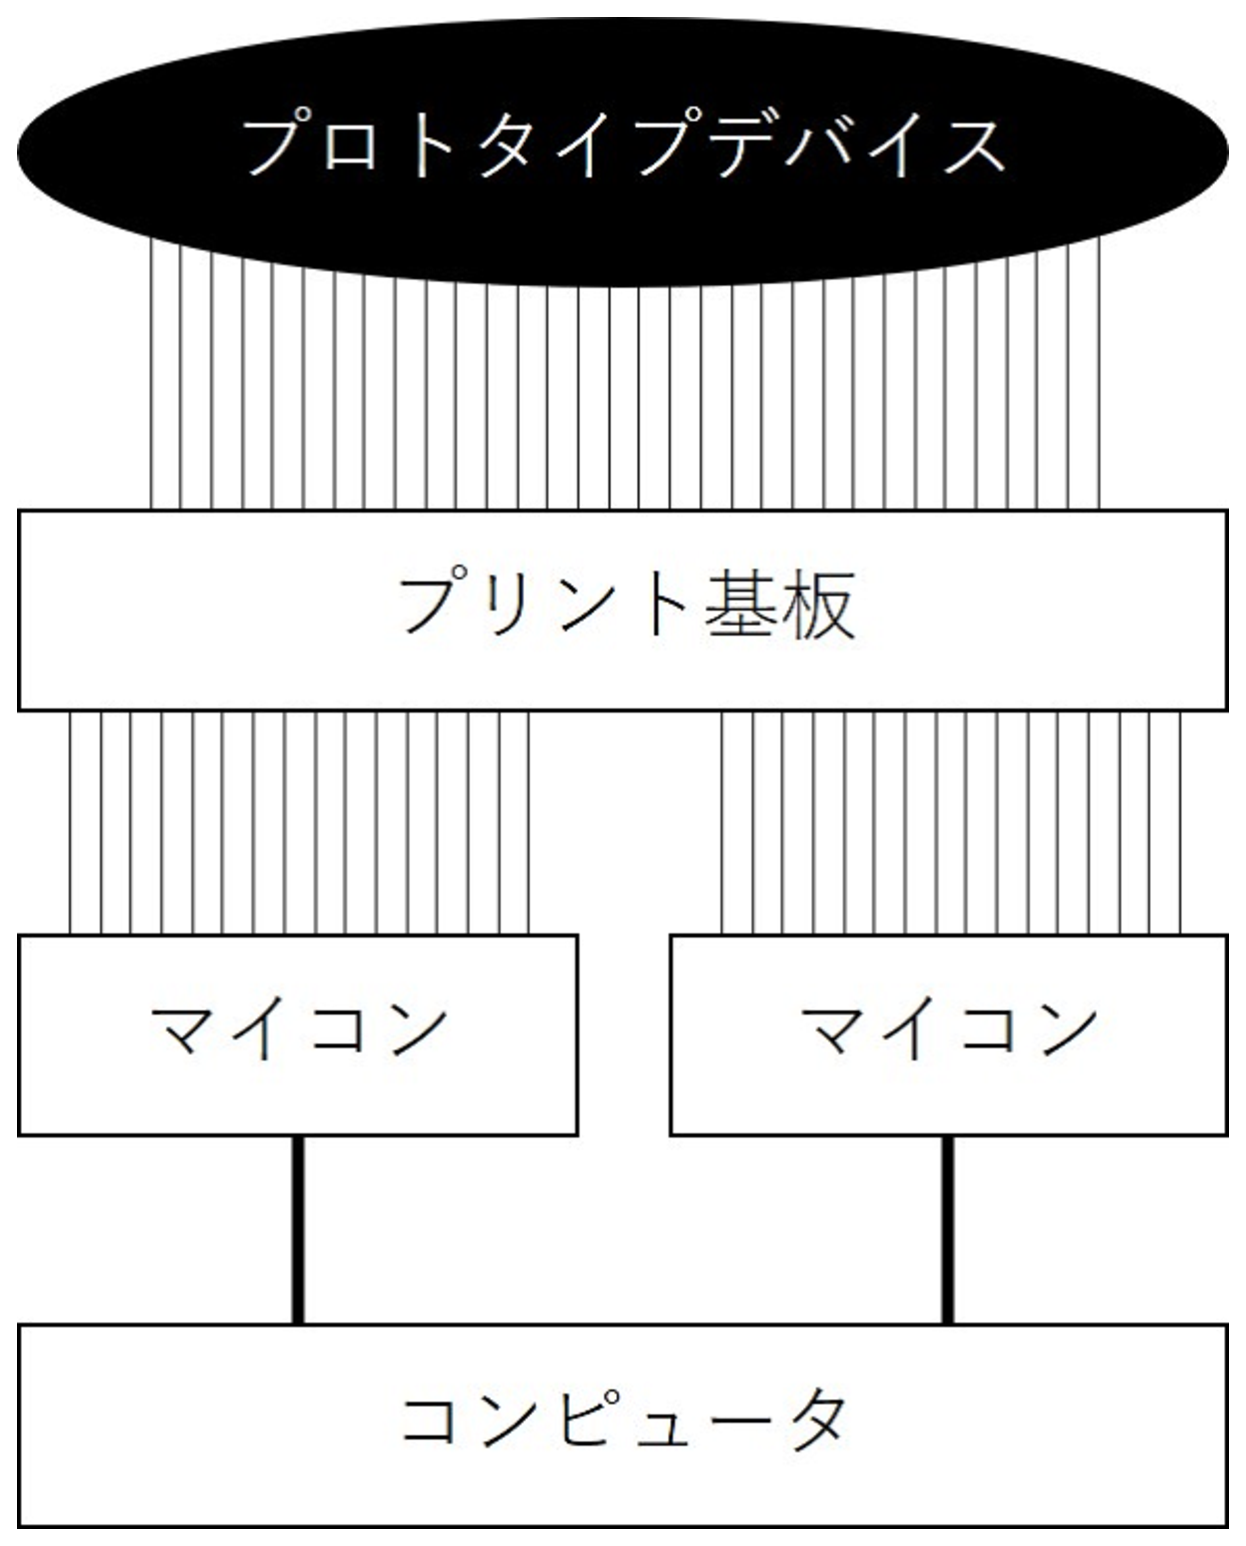
\includegraphics[width=1\linewidth]{figure/device.eps}
  \end{center}
  \caption{デバイス構成}
  \label{device}
\end{figure}

\begin{figure}[!t]
  \begin{center}
    \includegraphics[width=1\linewidth]{figure/met_over.eps}
  \end{center}
  \caption{プロトタイプデバイスの全体図}
  \label{met_over}
\end{figure}

\begin{figure}[!t]
  \begin{center}
    \includegraphics[width=1\linewidth]{figure/met_in.eps}
  \end{center}
  \caption{ヘルメットの内部}
  \label{met_in}
\end{figure}

\begin{figure}[!t]
  \begin{center}
    \includegraphics[width=1\linewidth]{figure/sensor.eps}
  \end{center}
  \caption{センサの実装方法}
  \label{sensor}
\end{figure}

\begin{figure}[!t]
  \begin{center}
    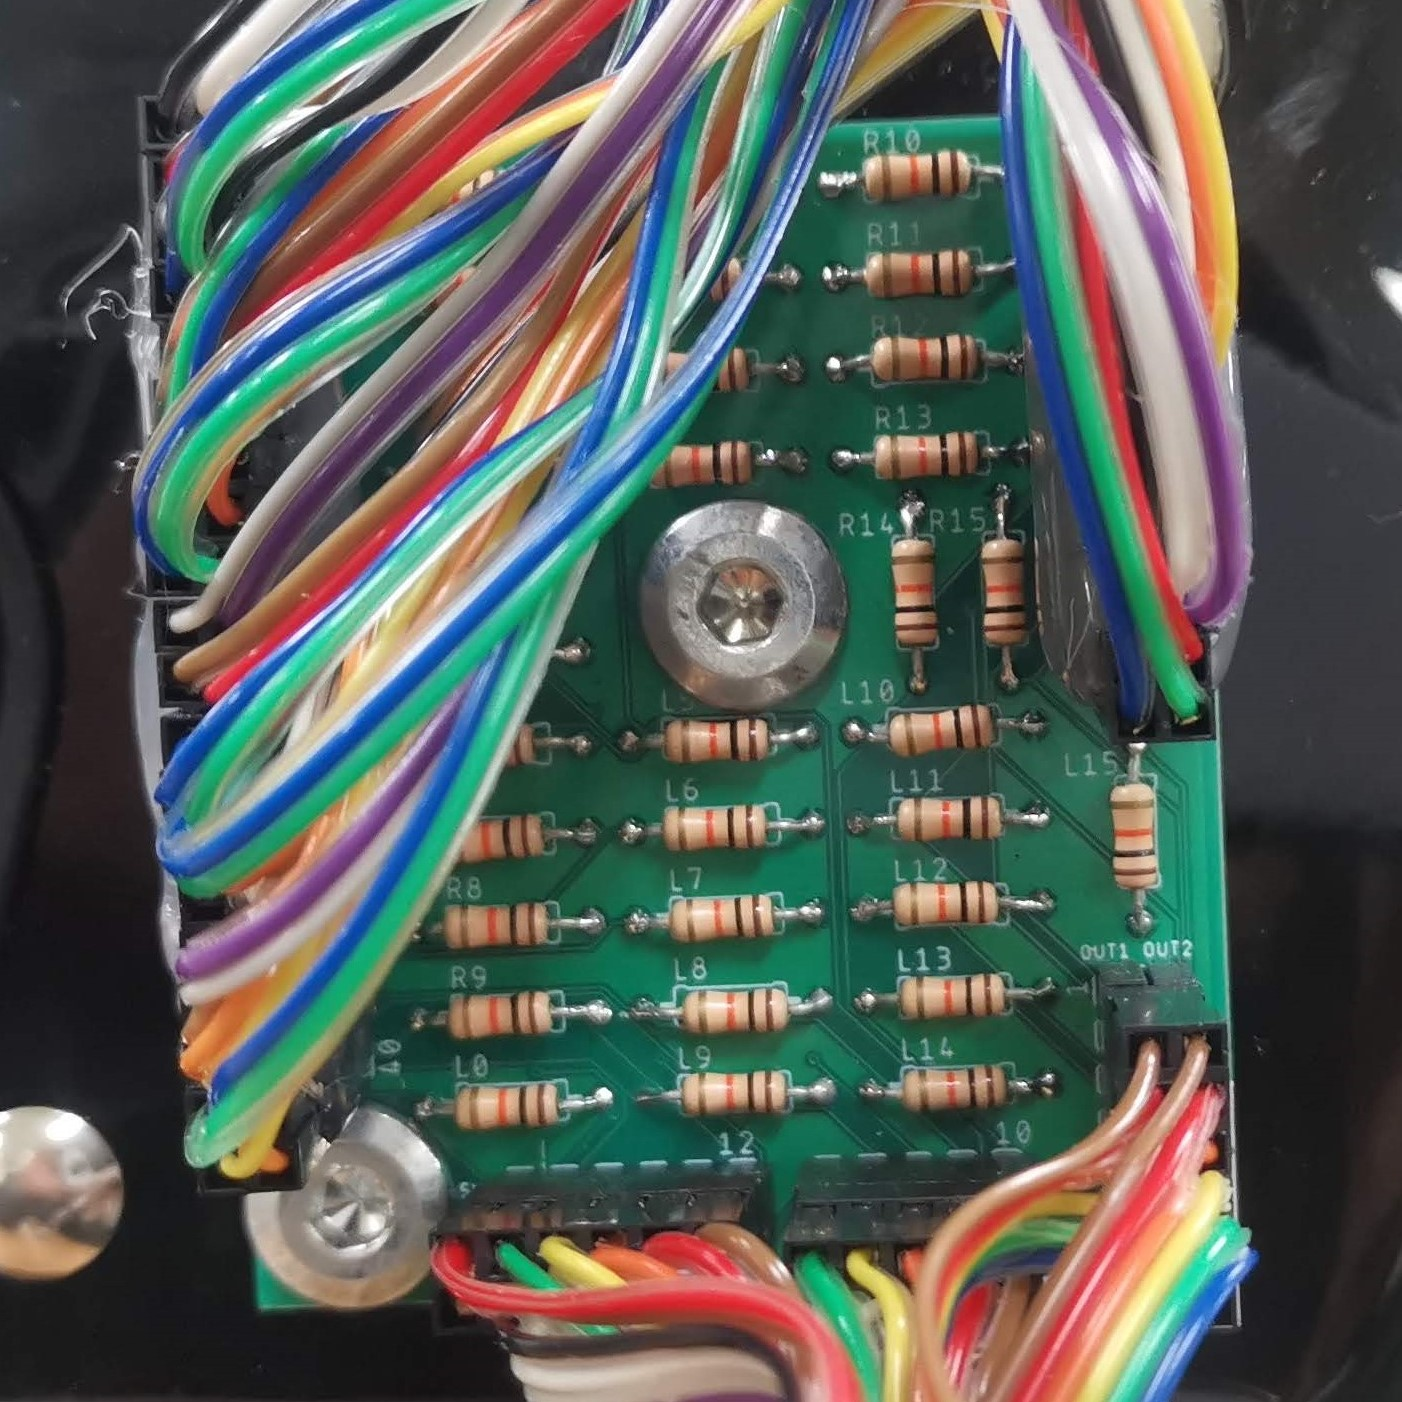
\includegraphics[width=1\linewidth]{figure/print.eps}
  \end{center}
  \caption{プリント基板}
  \label{print}
\end{figure}

\begin{figure}[!t]
  \begin{center}
    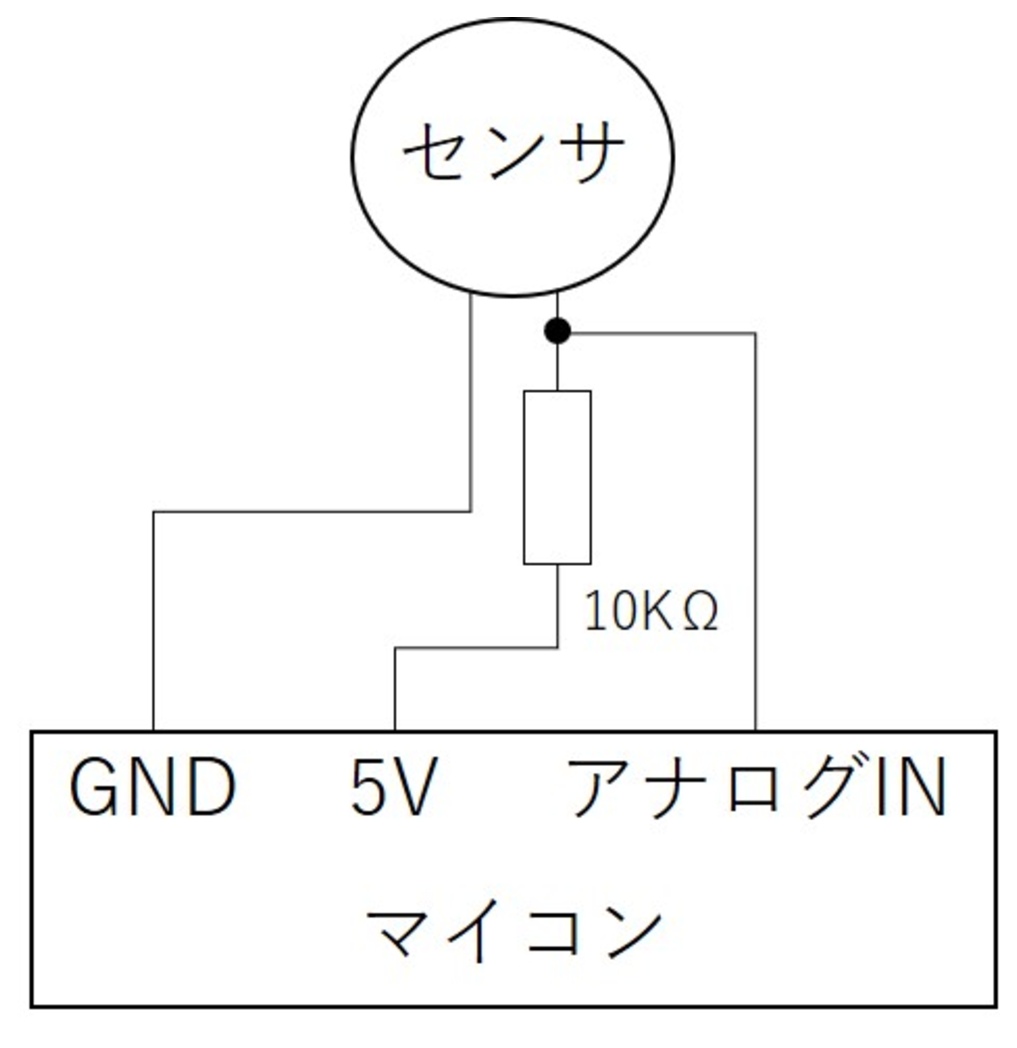
\includegraphics[width=1\linewidth]{figure/circuit.eps}
  \end{center}
  \caption{センサ1つあたりの回路図}
  \label{circuit}
\end{figure}

\subsubsection{ソフトウェア}
データの収集段階として,ArduinoIDEを用いてマイコンを制御し,Pythonでcsvとしてデータを採取するプログラムを作成した.次に解析段階としてPython上でcsvを読み出し,sklearn.covariance.MinCovDetを用いてマハラノビス距離を計算する.そして計算結果に対し,閾値を移動させながら比較,識別していくプログラムを実装した.\par
ここで用いたsklearn.covariance.MinCovDetとは,異常値に対して頑健な共分散行列の推定アルゴリズムであるMinimum Covariance Determinant(以下MCDと表記)を高速化した,Fast-MCDを実装したscikit-learnのライブラリである.次節では,このFast-MCDのアルゴリズムについて論じる.

\subsubsection{Fast-MCDのアルゴリズム}
マハラノビス距離は平均値ベクトルを用いて計算するため,異常値の影響を大きく受けてしまう.そこで,異常値に対して頑健な共分散行列の推定アルゴリズムであるMinimum Covariance Determinant(以下MCDと表記)が存在する.しかし,このアルゴリズムは膨大な計算量が必要であるため,実使用に耐えうるよう高速化されたアルゴリズムが,Fast-MCDである.Fast-MCDのアルゴリズムは次の通りである.\par
$x_i$を$p$次元確率ベクトルとしたとき,$X = {x_1, \ldots, x_n}$とし,$H_{old}\subset X$を$X$からランダムに抽出した大きさ$h$の$x_i$の集合とする.まず,$H_{old}$の平均ベクトルと共分散行列をそれぞれ$\hat{\mu}_{old}, \hat{\Sigma}_{old}$とし,$\hat{\Sigma}_{old}$の固有値$|\hat{\Sigma}_{old}|$を計算する.次に$\hat{\mu}_{old}, \hat{\Sigma}_{old}$を使ったマハラノビス距離を$X$の各要素に対して計算し,
\[
d(x_i) = \sqrt{(x_i-\hat{\mu}_{old})^{T}\hat{\Sigma}_{old}^{-1}(x_i-\hat{\mu}_{old})}
\]
とする.$d(x_i)$を小さいもの順に並べ,$d_{j:n}$をその中で$j$番目に大きいものとすると,次のようになる.
\[
d_{1:n}\leq \cdots\leq d_{j-1:n}\leq d_{j:n}\leq d_{j+1:n}\leq \cdots\leq d_{n:n}
\]
ここで,$d_{j:n}$を小さいもの順に$h$個取り出し
\[
H_{new} = {d_{1:n}, d_{2:n}, \ldots, d_{h:n}}
\]
とし,この$H_{new}$の平均ベクトル,共分散行列とその固有値$\hat{\mu}_{new}, \hat{\Sigma}_{new}, |\hat{\Sigma}_{new}|$を計算する.この作業を$|\hat{\Sigma}_{new}|=0$となるか,$|\hat{\Sigma}_{old}|-|\hat{\Sigma}_{new}|$が十分小さくなるまで繰り返す.この一連の流れから得られた平均ベクトルと共分散行列が,異常値に対して頑健なMCD推定量となる.

\section{評価}
\subsection{データ収集}
提案手法の有効性を確認するために,被験者5名(A$\sim$E,全員男性,平均年齢22歳)にプロトタイプデバイスを着用させ,サンプリングレート約30Hzでセンサデータを収集した.2秒間着用して取り外し,再び着用する試行を1セットとして合計10セット(2秒$\times$20回分)を収集した.ただし1度の着用に対して1つのデータが必要なので,以降この2秒間の平均値を使用することとする.データ収集は1人当たり1日最大4セットとし,複数日に渡って実施した.センサと頭部のさまざまな位置関係のデータを採取するために,セット間に30分以上の休憩時間を設けた.

\subsection{データ群の検証}
提案手法は距離に基づき装着者を識別する.すなわち,被験者ごとのデータ群に散らばりがなければ提案手法は成立しない.そのため収集したすべてのデータに対して主成分分析を行い,2次元に圧縮したデータを2次元平面上にプロットし,目視で確認できるようにした.その結果を図\ref{PCA}に示す.\par

\begin{figure}[!t]
  \begin{center}
    \includegraphics[width=1\linewidth]{figure/PCA.eps}
  \end{center}
  \caption{PCAによる分析結果}
  \label{PCA}
\end{figure}

被験者A,Eのデータ群は分散が小さく,更に他の被験者のデータ群と重なりが見られない.被験者B,Iのデータ群は分散が小さいものの,互いに重なりが見られる.被験者Cのデータ群は分散が大きいが,1つのデータが被験者Iのデータ群に近いことを除き,他の被験者のデータ群との重なりは見られない.被験者D,Hのデータ群は分散が小さいが,互いにかなり重なっている.被験者F,Gのデータ群は分散が大きいものの,他の被験者のデータ群との重なりは見られない.\par
以上の結果は2次元に主成分分析しているため,データ量が大きく損失している.その点を考慮した上で,ヘルメット内部に搭載した圧力センサのデータから,距離に基づき装着者を識別できると判断した.次節では実際の判別結果について論じる.

\subsection{提案手法での識別結果}
識別結果の評価指標として,FAR,FRR,EERを用いる.FAR(False accept rate:他人受入率)とは他人のデータを本人と誤って認証してしまうことであり,FRR(False reject rate:本人棄却率)は本人のデータを他人と誤って拒否してしまうことである.閾値を小さくするほどFRRが増加し,閾値を大きくするほどFARが増加する.これらはトレードオフの関係であり,FARとFRRが同値になるときの値をEER(Equal error rate:等価エラー率)と呼ぶ。このEERが小さいほど精度が良いとされる.データセットに対し,被験者ごとに5分割交差検証を行い指標を計算した.\par
提案手法を用いて識別した結果を図\ref{EER}および,小数第二位を四捨五入したEERの値を表\ref{EER_num}に示す.ここで,Totalは全体での結果を示す.この値は全被験者の平均値を求めたものである.

\begin{figure}[!t]
  \begin{center}
    \includegraphics[width=1\linewidth]{figure/EER.eps}
  \end{center}
  \caption{被験者ごとの判別結果}
  \label{EER}
\end{figure}

\begin{table}[htb]
  \center
  \begin{tabular}{|c|c|} \hline
    被験者 & 値(約) \\ \hline \hline
    A & 0\% \\
    B & 10\% \\
    C & 5\% \\
    D & 7\% \\
    E & 1\% \\
    F & 7\% \\
    G & 1\% \\
    H & 5\% \\
    I & 0\% \\ \hline
    Total & 7.8\% \\ \hline
  \end{tabular}
  \caption{被験者ごとのEER}
  \label{EER_num}
\end{table}

\section{考察}
表\ref{EER_num}より被験者A,HのEERは0\%である.これは,検証に用いたデータセットでの識別が完全にできたということを意味している.しかし図\ref{PCA}では,被験者Aは他の被験者のデータ群との重なりがなかったものの,被験者Hは重なりが見られる.これは2次元に圧縮した際のデータの損失による影響だと考えられる.次いで結果が良かったのは被験者E,Gの1\%だった.ここで図\ref{EER}より,被験者EのみEERの得られた閾値が大きいことがわかる.その一方,図\ref{PCA}では被験者Eのデータ群はかなり隔離されている.これも同様にデータの損失の影響であり,主成分分析で丸められているが,生データでは外れ値が存在したために閾値が大きくなったと考えられる.他の被験者でも同様に,データ群の重なりから期待されるEERと結果が異なる場合があったが,いずれもデータの損失による影響だと考えられる.また,全体ではEERが7.8\%という結果であった.被験者ごとのEERに差が見られたことから,さらなる精度の向上を目指すことが可能だろう.\par
提案手法ではマハラノビス距離を用いて識別を行うため,学習データ数をさらに増やすことで精度の向上が見込まれる.その一方で,距離が同じ場合は識別が不可能となってしまう.その場合,提案手法とは別の手法で識別を行う必要がある.具体的にはヘルメットを装着する一連の流れを時系列データとして取得し,その特徴により識別を行うなどの手法が考えられる.この手法が有効であるか,今後実験していく必要がある.

\section{おわりに}
本研究では,圧力センサを内部に取り付けたヘルメットを着用することで頭部の形状を計測し,頭部形状の個人差から二輪車の所有者本人を識別する手法を提案した.評価実験より個人ごとにはEERが0\%$\sim$10\%,全体では約7.8\%という結果が得られた.この結果より,本手法は個人識別手法として有効であると考えられる.今後はさらなるデータ採取を行い,実環境での提案手法の評価を行う.また,利用者のデータ群に差がないときの個人識別方法を定義し,検証していきたい.

\bibliography{../references}
\bibliographystyle{junsrt}

\end{document}
